% METODOS
El estudio de la distribución de las direcciones de arribo de los eventos es una herramienta importante para obtener información sobre el origen de los RCs . Las irregularidades sobre el flujo casi isotrópico de los RCs, en un rango de energía, pueden deberse a  zonas del espacio donde se producen más RCs que en otras, estas irregularidades se conocen como anisotropías. 

El análisis de anisotropías a grandes escalas angulares suele ser hecho sobre las irregularidades de la distribución de eventos en ascensión recta $\alpha$, ya que el arreglo principal tiene una exposición direccional en función de esta coordenada casi constante \cite{referencia_anis}.

\section{Cálculo de los coeficientes de Fourier para el análisis de anisotropía en ascensión recta}

Las anisotropías son variaciones pequeñas por lo que eliminar todo factor espurio en el análisis es importante. Para obtener la amplitud de la misma en ascensión recta, se estudia la frecuencia sidérea ($f_{sid}=366.25\,$ ciclos/año) \cite{taborda}. Los errores sistemáticos debido a la modulación de eventos por el clima u otros errores propios de la adquisición de datos, aparecen en la frecuencia solar  ($f_{sid}=365.25\,$ ciclos/año), por lo que se debe tener en consideración el análisis de esta frecuencia. La frecuencia anti-sidérea ($f_a=364.25\,$ ciclos/año) es una frecuencia que puede indicar efectos sistemáticos en la amplitud de la anisotropía en la frecuencia sidérea \cite{farley1954sidereal}. La mezcla entre modulaciones diarias y anuales induce bandas laterales ubicadas a $\pm1\,$ciclo/año con respecto a la solar \cite{taborda}. Por estos motivos se toman estas frecuencias  como referencia.

  \subsection{Variaciones relativas de los hexágonos} \label{peso_hexagonos}

Para corregir las variaciones de la exposición del observatorio, podemos definir un peso  $w_i$ por cada evento $i$, que corrige la variación  $\Delta N_{cell}(\alpha^0)$ en función de la ascensión recta del cenit del observatorio $\alpha^0$ durante el rango de tiempo estudiado. Estas variaciones pueden deberse al crecimiento del arreglo a través de los años,  por caídas en la comunicación del observatorio con los SDs u otros motivos. 

El factor $\Delta N _{cell}(\alpha^0)$ tiene en cuenta que la exposición  direccional  el observatorio no es uniforme en tiempo sidéreo.  Se obtiene sumando el número de celdas durante el periodo de medición, en cada segmento de $\alpha^0$ y luego se normaliza con el valor medio de los segmentos.

Para calcular estos pesos $w_i$, se sigue el algoritmo presentado a continuación:
     
      \begin{enumerate}
        \item Se establecen una frecuencia $f$  y un rango de tiempo a estudiar. Por ejemplo, se desea estudiar la frecuencia solar entre el 1 de Enero del 2014 a las 12:00:00 GMT y el 1 de Enero del 2020 a las 12:00:00 GMT.

        \item Cada dato del registro de hexágonos, tomado en un momento $t$ durante el rango seleccionado, se clasifica según la cantidad de horas desde un momento de referencia $t_0$. Esta referencia $t_0$ se tomará como el 1 de Enero del 2005 a las 00:00:00 GMT, o  $21\,$hs del 31 de Diciembre del 2004, según la hora local de Malargüe.

        \item Podemos asociar una coordenada angular $h$ a $t$  y $f$  utilizando la siguiente expresión:
         \begin{equation}
          h = (t-t_0) \times \frac{360^o}{24\text{hs}} \times\frac{f}{f_{Solar}} + h_0
          \label{eq:h_horas} 
        \end{equation}
        El factor $\nicefrac{f}{f_{Solar}}$ sirve para hacer un cambio de escala temporal entre los periodos de distintas frecuencias. Se usa como referencia la $f_{Solar}$ dado que las horas (solares) se basan en esta frecuencia, y el valor de $h_0=31.4971^o$ representa la ascensión recta del cenit del observatorio en el momento utilizado como referencia.
        
        \item  Para simplificar el cálculo del peso de los hexágonos, se divide los $360^o$ de la ascensión recta en $L$ segmentos de $\nicefrac{360}{L} ^o$ cada uno. Para clasificar un dato se  toma  el valor $h$  y se calcula
        \begin{equation}
          h' = h\, mod \,360 %=  h - 360\Big \lfloor \frac{h}{360} \Big \rfloor
          \label{eq:h_primado}
        \end{equation}
        donde la función $mod$ representa la función módulo que devuelve un número real positivo. Con el valor de $h'$ del dato, se asigna el mismo al segmento $k$ que le corresponde, mediante la siguiente expresión
        \begin{equation}
          k = \bigg \lceil \frac{h'}{360}\times L \bigg \rceil
        \end{equation}
        donde $\lceil a \rceil$ representa la función techo \footnote{La función techo da como resultado el número entero más próximo por exceso}. Por ejemplo, si optamos por $L=24$ y un dato en particular resulta con  $h=395\,^o$, esto implica que $h'= 35^o$ y que $k=\lceil 2.333 \rceil=3$, por lo tanto, este registro corresponde al segmento en la $3^{a}$ posición.

        \item Una vez clasificados todos los datos del registro de hexágonos, se calcula la suma  $N_{hex, j}$ de los datos que cayeron un segmento $j$ dado. Para definir la variación relativa de hexágonos  $\Delta N_{cell,k}$ de un segmento $k$ en particular, necesitamos la media de hexágonos por segmento $ \langle N \rangle$  para normalizar las variaciones.
       \begin{align}
         \langle N \rangle &= \sum^{L}_{i=1} \frac{N_{cell, i}}{L}  \qquad
         \Delta N_{cell,k} = \frac{N_{cell, k}}{\langle N \rangle}  \label{epepe}
       \end{align}

      \end{enumerate}
 En la Fig.\ref{fig:pesos_referencia} se muestran las variaciones relativas de los hexágonos en función de la ascensión recta del cenit del observatorio para las frecuencias mencionadas. Este análisis fue realizado en el marco del trabajo \cite{referencia_pesos} con eventos del periodo 2004-2017. 



       En la Fig.\ref{fig:pesos_ejemplo} se observan los valores obtenidos de $\Delta N_{cell,k}$  con el código escrito para este trabajo, en función de la ascensión recta del cenit  para $L=288$ segmentos. Se analizó el conjunto de datos  utilizado para obtener los resultados la Fig.\ref{fig:pesos_referencia}, con el fin de validar dicho código. Los datos se analizaron desde el 1 de Enero del 2004 a las 00:00:00 GMT  hasta el 1 de Enero del 2017 a las 00:00:00 GMT. Se  observa que los resultados obtenidos son compatibles con la Fig.\ref{fig:pesos_referencia}
      
      \begin{figure}[H]
          \centering
              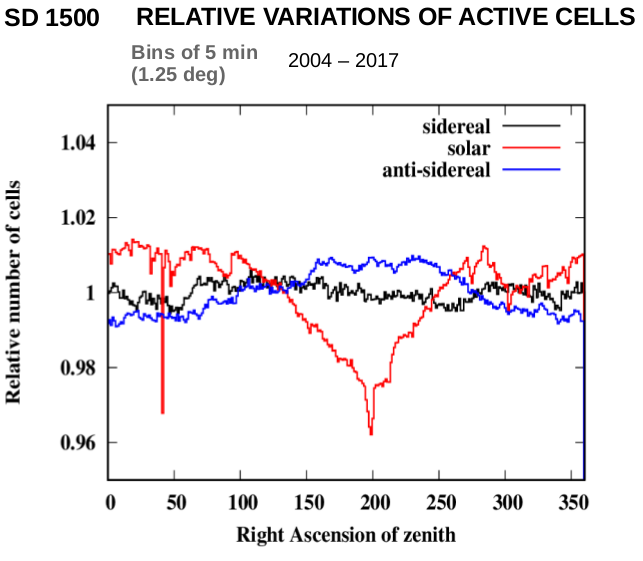
\includegraphics[width=0.5\linewidth]{pesos_referencia.png}  
              \caption{Valores de $\Delta N_{cell, k}$ en el rango 2004-2017 para distintas frecuencias obtenidas en el trabajo \cite{referencia_pesos}.}
              \label{fig:pesos_referencia}
        \end{figure}

       \begin{figure}[H]
          \centering
              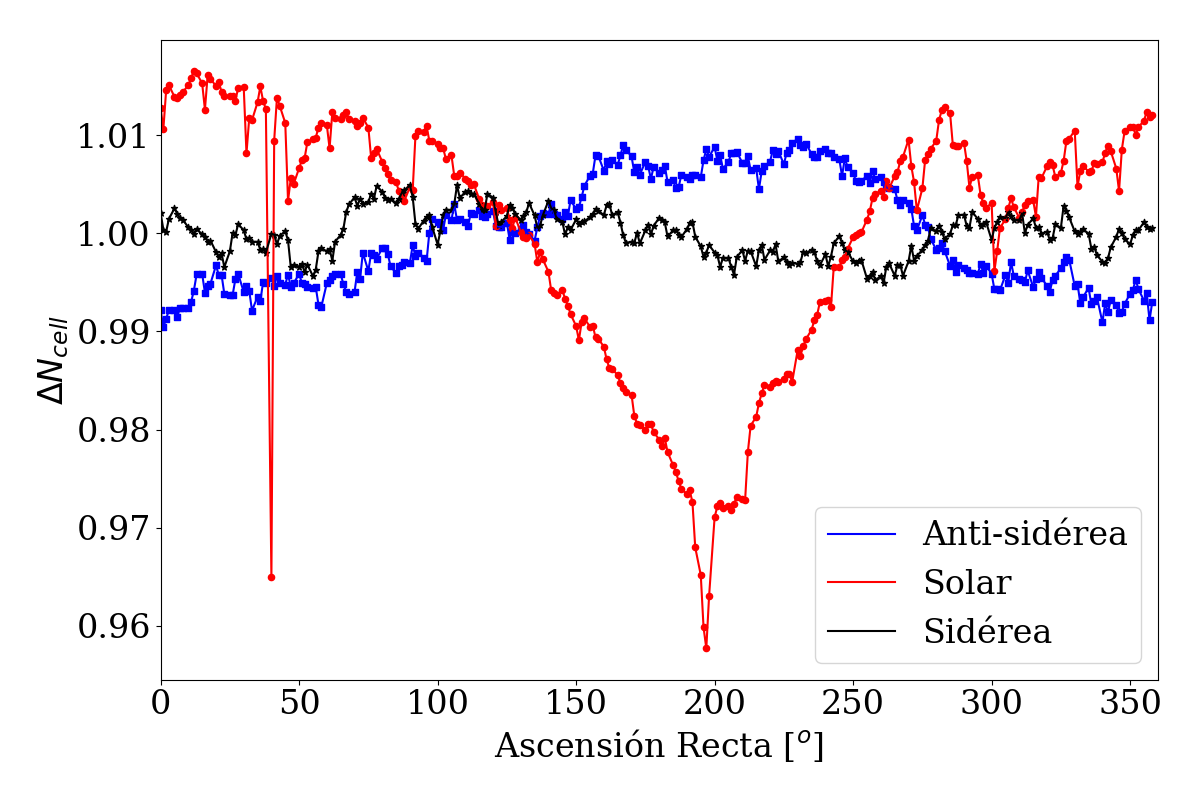
\includegraphics[width=0.75\linewidth]{weigths_2020.png}
              \caption{Valores de $\Delta N_{cell, k}$ en el rango 2004-2017 para distintas frecuencias utilizando el código escrito en este trabajo.}
              \label{fig:pesos_ejemplo}
        \end{figure}

    Para una representación fiel entre los registros de los hexágonos y los pesos de los eventos, se optó por clasificar los datos de los hexágonos en $288$ segmentos, donde cada segmento tiene un ancho de $1.25^o$. Esto es conveniente ya que la actualización del registro de hexágonos se realiza una vez  cada $5\,$min como se menciona en la sección \ref{hexagonos_rate}. Esta tasa de actualización es equivalente a decir que la adquisición se realiza cada vez que el cenit del observatorio barre  $1.25^o$ en ascensión recta sobre la esfera celeste.


  \subsection{Cálculo de Rayleigh en ascensión recta para una frecuencia dada} \label{rayleigh}

  Un procedimiento para estudiar anisotropías en la direcciones de arribos de los RCs es realizar un análisis de Fourier en ascensión recta $\alpha$. La distribución en ascensión recta $\alpha$ del flujo de RCs $I(\alpha)$ que llega al arreglo principal puede caracterizarse por las amplitudes $r_k$ y fases $\phi_k$ de su expansión en serie de Fourier al $k-$ésimo orden. 

  \begin{equation}
    I(\alpha) = I_0 \bigg ( 1+ \sum^\infty_{k=1} r_k\cos{[k(\alpha - \phi_k)]} \bigg) = I_0 \bigg ( 1+ \sum^\infty_{k=1} a_k\cos{k\alpha} +  b_k\sin{k\alpha} \bigg ) 
  \end{equation}
  donde $a_k=r_k\cos k\phi_k$ y $b_k=r_k\sin k \phi_k$, y $I_0$ es el flujo medio. La distribución $I(\alpha)$ puede obtenerse a partir de la distribución de direcciones de arribo de los eventos observados.  En este trabajo, suponiendo que existieron $N$ eventos en el rango analizado, se considera que los mismos tienen una distribución en ascensión recta del tipo $\nicefrac{dN}{d\alpha}= \sum^N_{i=1} \delta(\alpha - \alpha_i)$ \cite{taborda}. 

  Como se mencionó anteriormente, los análisis en ascensión recta están asociados a la frecuencia sidérea. Para realizar el análisis de los eventos en cualquier frecuencia arbitraria, es necesario modificar $\alpha$ por $\tilde{\alpha}$. Esta nueva variable tiene la forma como se utiliza en el trabajo \cite{taborda}:
  \begin{equation}
    \tilde{\alpha} = 2\pi f_x t_i + \alpha_i - \alpha_i^0(t_i) \label{ra_mod}
  \end{equation}
  donde $f_x$ es el frecuencia arbitraria a estudiar, $t_i$ es el momento en que ocurrió el evento y $\alpha_i^0(t_i)$ es la ascensión recta del cenit del observatorio en el momento del evento. Si la frecuencia a analizar es la sidérea, el análisis con $\alpha$ y $\tilde{\alpha}$ arrojan los mismos parámetros $r_k$ y $\phi_k$.

 Clasificando a los eventos mencionados en la sección \ref{specs} según el valor de la ascensión recta y considerando que todos los eventos tienen un peso uniforme de $w_i=1$, se dicen que los eventos fueron analizados \textit{sin pesos}, donde no consideramos la corrección de la exposición. En caso contrario, se habla de análisis \textit{con pesos} de los hexágonos  y estos pesos se calculan como se menciona en la sección anterior.

  Para realizar el análisis de frecuencias de los eventos, en el $k$-ésimo orden en la expansión de Fourier, se siguen los siguientes pasos.

        \begin{enumerate}
        \item Fijando un rango de tiempo y un rango de energía en el cual se desea estudiar la anisotropía, se establece una frecuencia en particular $f$ a analizar. Siguiendo el ejemplo de la sección anterior, se analiza la frecuencia solar entre el 1 de Enero del 2014 a las 12:00:00 GMT y 2019 hasta el 1 de Enero del 2020 a las 12:00:00 GMT.

        \item Con los eventos ya filtrados según el criterio de la sección \ref{filtro}, asigno cada evento $i$ un valor $h_i$, definida en la Ec.\ref{eq:h_horas}

        \item En caso de considerar los pesos de los hexágonos, para asignar el peso correspondiente al evento, se asocia a un segmento $k$, calculado en la sección \ref{peso_hexagonos}, mediante el valor de $h'_i$ definido en la Ec.\,\ref{eq:h_primado}. Luego, el peso asignado $w_i$  al evento $i$ es: $ w_{i}= (\Delta N_{cell,k})^{-1}$, caso contrario, se toman que todos los eventos tiene $w_i=1$.
        
        \item Para el análisis en frecuencias, a partir del valor de $h_i$ se asigna el ángulo $\tilde{\alpha}_i$ definida en la Ec.\ref{ra_mod}. La implementación en el código es de la siguiente manera: 
        \begin{equation}
         \tilde{\alpha}_i = 2\pi \frac{h_i}{360^o} + \alpha_i -\alpha^0_{i}
        \end{equation}
        donde $\alpha_i$  representa la ascensión recta del evento y $\alpha^0_{,i}$ la ascensión recta en el cenit del observatorio en el momento del evento. Cabe resaltar que la información de la frecuencia que se está estudiando se encuentra en el valor de $h$. Si la frecuencia a estudiar fuera la sidérea, el término $2\pi \frac{h}{360^o} $ seguiría el cenit del observatorio, por lo que este término sería equivalente a $\alpha^0_{i}$, por lo tanto en esta frecuencia $ \tilde{\alpha}_i =\alpha_i$ como es de esperarse. 
        
        \item Para calcular los coeficientes de Fourier del k-ésimo armónico $a_k$ y $b_k$, se siguen los siguiente pasos:
        \begin{enumerate}
          \item Por cada evento  $i$ se calculan los siguientes valores:
          \begin{equation}
             a_{ik}' = {w_i}\cos k\tilde{\alpha}_i \qquad
             b_{ik}' = {w_i}\sin k\tilde{\alpha}_i
         \end{equation}
         \item Una vez que se obtuvieron los valores de $a_{ik}'$ y $b_{ik}'$ para todos los eventos en el rango de tiempo estudiado, se calculan los coeficientes definidos en el trabajo \cite{analisis_fourier} mediante:
         \begin{alignat}{3}
          \mathcal{N} &= \sum^{Eventos}_i w_i \qquad
            a_k = \frac{2}{\mathcal{N}} \sum^{Eventos}_i a_{ik}' \qquad
            b_k = \frac{2}{\mathcal{N}} \sum^{Eventos}_i b_{ik}'  
         \end{alignat}
        \end{enumerate}
        \item Con los coeficientes es posible calcular la amplitud de la frecuencia estudiada $\tilde{r}$ y la fase $\phi$. Otros parámetros calculados para el análisis son la probabilidad $P(\tilde{r})$  y $r_{99}$. 
        \begin{alignat}{3}
            \tilde{r}_k &= \sqrt{a_k^2 +b_k^2}                       \qquad &&   \phi_k&&= \frac{1}{k}\arctan\frac{a_k}{b_k}\\
          P(\tilde{r}_k)&= \exp(-\mathcal{N}\frac{\tilde{r}_k^2}{4})\qquad &&   r_{99}&&= \sqrt{\frac{-4\log(0.01)}{\mathcal{N}}}
        \end{alignat}
        Cabe resaltar que el $r_{99}$ depende solamente de los pesos de los eventos que se está estudiando. La interpretación  de este valor es cual es la probabilidad de tener una amplitud mayor como una fluctuación de una distribución isotrópica sea del $1$\%
        %., y el valor de amplitud $r_{99}$ para que dicha probabilidad sea del $1$\%.
      \end{enumerate}

    Una forma de validar el código para el análisis de anisotropía es comparar los resultados del código con los obtenidos en otros trabajos \cite{taborda}. En la Fig.\ref{fig:sin_pesos_referencia} se muestra el análisis hecho sobre el mismo conjunto de eventos. Estos eventos fueron adquiridos con el disparo estándar desde el 1 de Enero del 2004 a las 00:00:00 GMT  hasta el 1 de Enero del 2017 a las 00:00:00 GMT. Se consideraron los eventos por encima de $8\,$EeV que además cumplan las condiciones dadas en la sección \ref{filtro}.  En esta figura que los resultados obtenidos en \cite{taborda} y con el código utilizado por este trabajo son indistinguibles. 

      \begin{figure}[H]
        \centering
        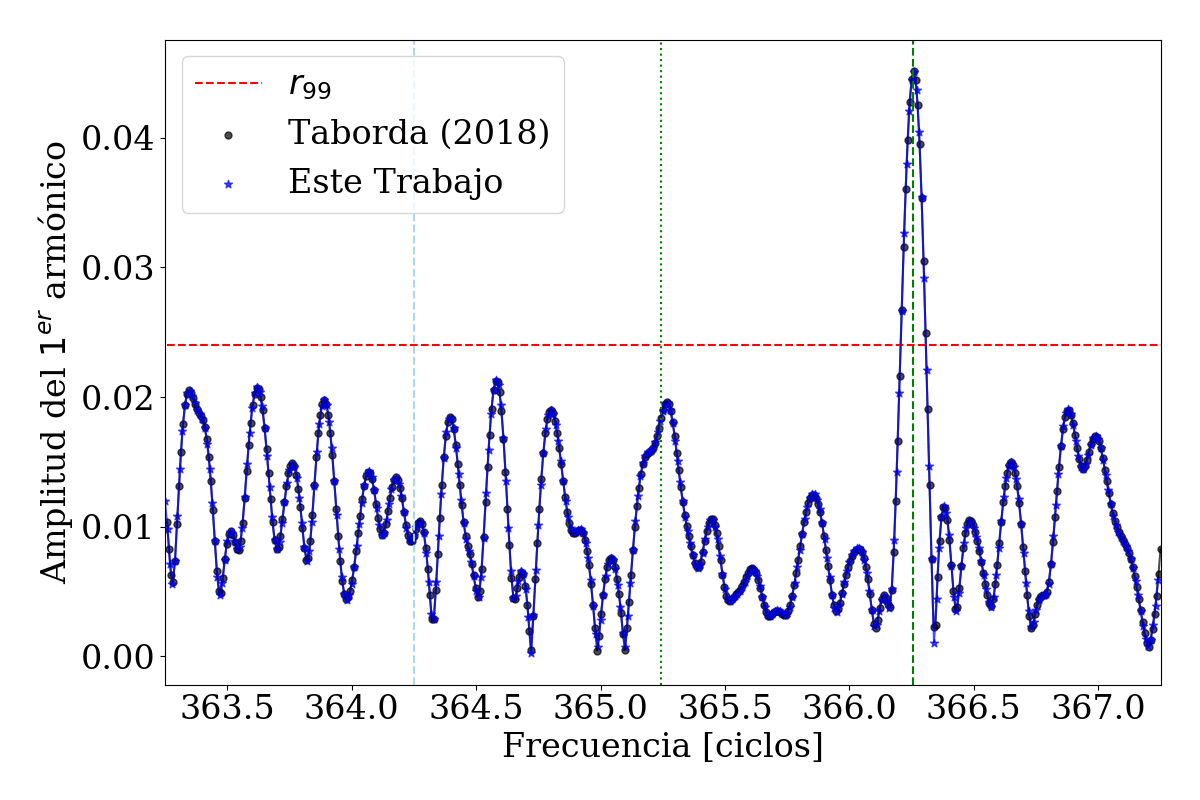
\includegraphics[width=0.75\linewidth]{sin_pesos_referencia_8_EeV.png}
        \caption{Comparación entre los análisis de anisotropía hechos para el mismo conjunto de datos, con el código de \cite{taborda} y con el código escrito para este trabajo.}
        \label{fig:sin_pesos_referencia}
      \end{figure}
